 \section{Architektura}
 Cílem této práce je vytvoření programu, který bude schopen detekovat anomální provoz v IoT sítích. 
 Vzhledem k hardwarovým omezením, které můžou na IoT branách nastat, je architektura navržena tak, aby
 měla co nejmenší nároky na dostupné prostředky. Schéma nasazení detekčního systému se nachází
 na obrázku \ref{obr.deploy-arch}
 
 \begin{figure}[ht]
   \begin{center}
   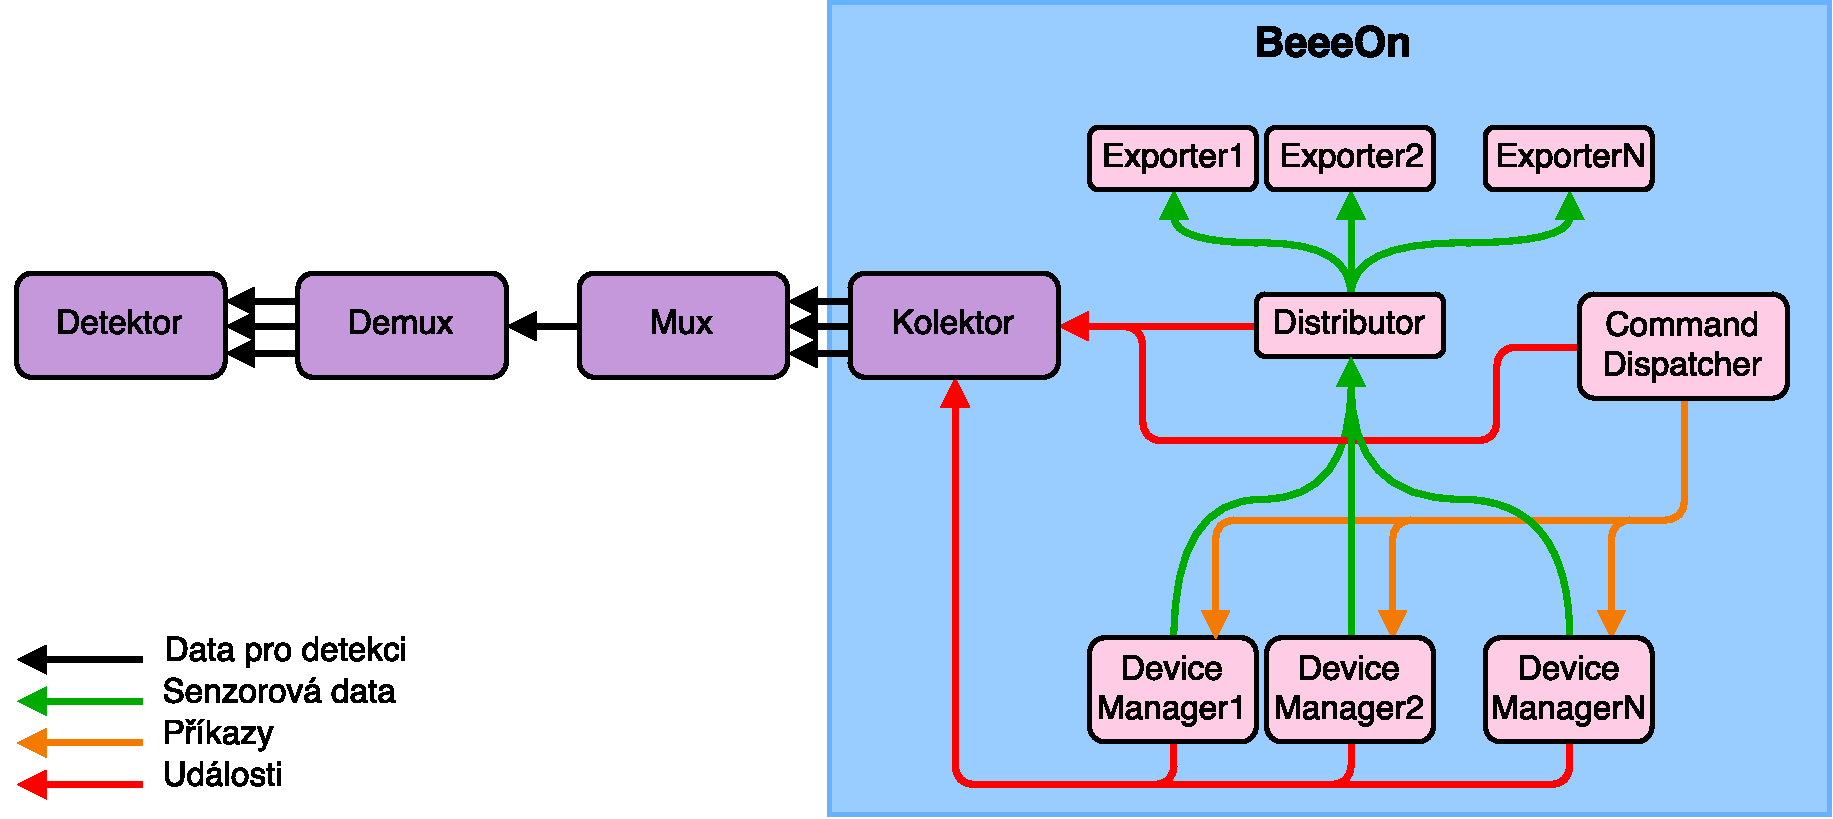
\includegraphics[scale=0.41]{pictures/deploy-arch}
   \caption{Architektura detekčního systému}
   \label{obr.deploy-arch}
   \end{center}
   \end{figure}
 
 Implementace BeeeOn brány obsahuje pro zpracování senzorových dat následující komponenty:
 \begin{itemize}
  \item \textbf{DeviceManager}:
    komponenta definovaná pro každý senzorový protokol, která implementuje veškerou komunikaci
    a zpracování dat
    
  \item \textbf{Distributor}:  
  přijímá data od \textit{DeviceManageru}, která nasledně předává příslušnému \textit{Exporteru}
  
  \item \textbf{Exporter}:
  implementuje protokol, kterým jsou data odesílány z brány
  
  \item \textbf{CommandDispatcher}:  
  komponenta, která přijímá uživatelské příkazy a distribuuje je cílovým komponentám
  
 \end{itemize}
 
 Každá z komponent v BeeeOn bráně navíc využívá návrhový vzor Observer, pomocí kterého jsou
 definovány události poskytující informace o každé komponentě. 
 Tímto způsobem bude vytvořený kolektor zíkávat data o provozu, která
 převede do fomátu UniRec (Unified Record) a pomocí systému NEMEA je odešle k analýze.
 
 Exportované informace o provozu bude přijímat detektor, který následně provede jejich zpracování a 
 vyhodnocení stavu. Všechny vytvořené komponety vytvořené pro detekci budou používat rozhraní 
 NEMEA. Díky tomu bude možné komponenty flexibilně provozovat na jednom nebo více různých zařízeních.
 Oddělené nasazení je důležité zejména pro brány s omezenými prostředky, které mohou provádět 
 pouze export dat a o vyhodnocení se bude starat odlišné zařízení s dostatečným výkonem. V případě 
 provozování více bran lze brány používat jako exportéry a veškerá získaná data zpracovávat 
 centrálně. 
 
 Kolektor pro každou událost vytvoří samostnatné výstupní rozhraní. Protože událostí může být 
 velké množství, tak bude vytvořen modul \textit{Mux}, který všechny výstupní rozhraní spojí do jednoho. 
 Pro zpětné rozdělení na jednotlivá rozhraní budou dloužit modul \textit{Demux}. Tyto moduly budou velmi užitečné
 zejména v případě kdy kolektor a detektor budou na rozdílných síťových prvcích, protože údaje 
 o provozu budou přenášeny přes počítačovou síť a bude vyžadováno zabezpeční všech odchozích
 rozhraní. S využítím \textit{Mux} a \textit{Demux} modulů bude stačit zabezpečit pouze jedno sjednocené rozhraní. 
 
 Výhodou návrhu řešení je flexibilita a modularita. Každá komponenta vždy samostatně pokrývá pouze jednu
 část detekčního systému a se díky NEMEA se každá z nich může nacházet na různých síťových prvcích. Zároveň
 v případě potřeby lze vytvořit další moduly, které budou rozšiřovat stávající funcionalitu.
 Podrobnější popis návrhu nově vytvořených komponent detekčního systému se nachází v následujících kapitolách.
 
 \section{Kolektor}
 Úkolem kolektoru bude sběr dostupných dat a jejich odeslání k následné analýze. Informace o 
 provozu budou sbírány z jednotlivých komponent BeeeOn brány, které jsou zpřístupňovány pomocí 
 návrhového vzoru Observer. Z tohoto důvodu bude kolektor vždy přímou součástí BeeOn brány. 
 Návrh struktury kolektoru je na obrázku \ref{obr.modelTrid}
 
 \begin{figure}[ht]
   \begin{center}
   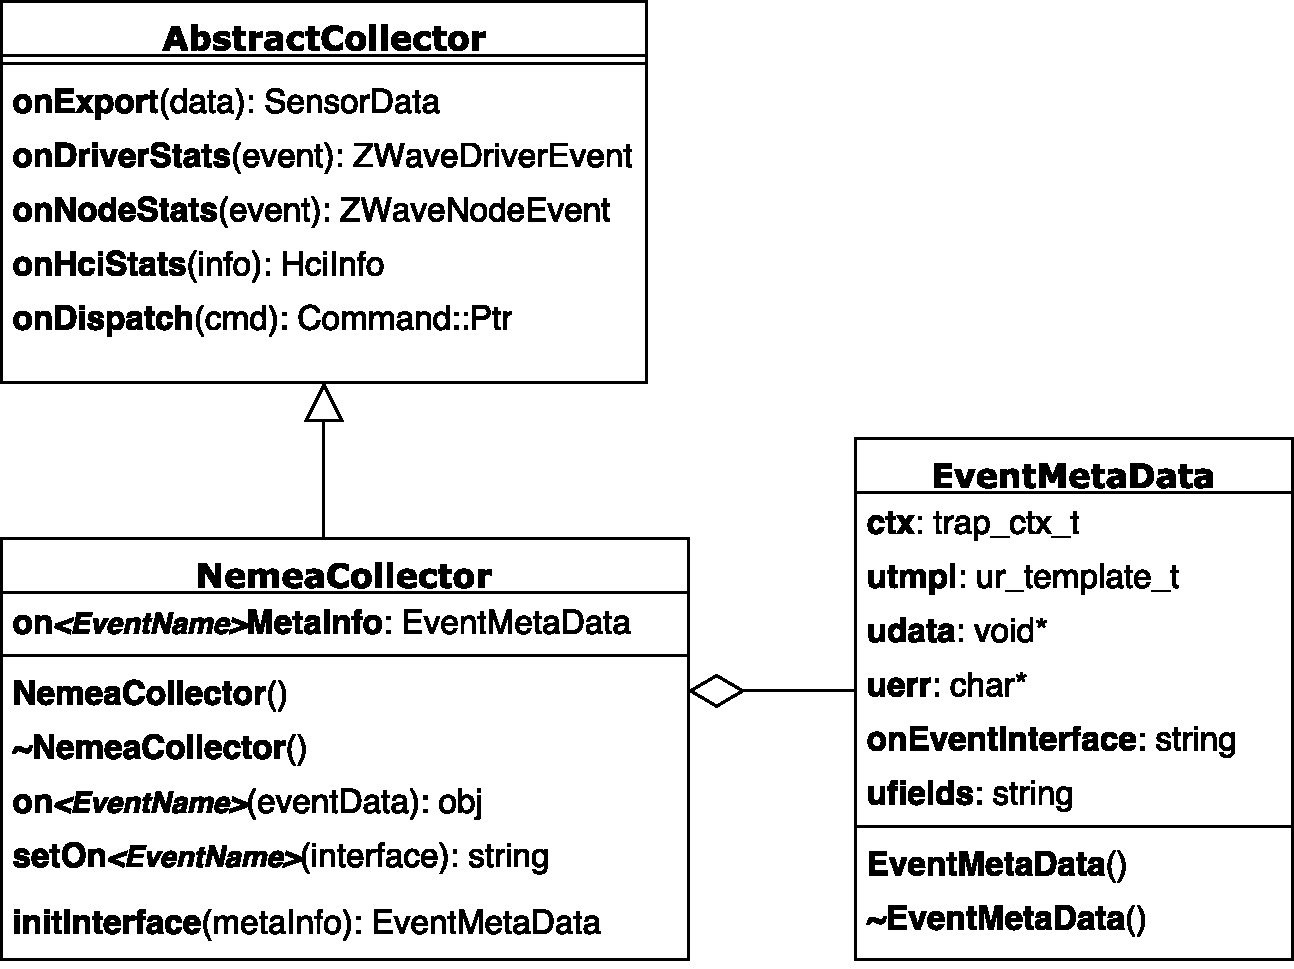
\includegraphics[scale=0.5]{pictures/modelTrid}
   \caption{Návrh kolektoru provozních dat}
   \label{obr.modelTrid}
   \end{center}
   \end{figure}
 
 AbstractCollector, je třída vytvořená v projektu BeeeOn, které shromažďuje všechny dostupné události.
 V současné době jsou k dispozici následující události:
 \begin{itemize}
  \item \textbf{onExport}:
   reprezentuje hodnoty dat přicházejících ze senzorů, která jsou odeslána vždy po jejich příjmu
   
  \item \textbf{onDriverStats}:
   v pravidelných intervalech generuje statistiky o Z-Wave sítí dostupné na komunikačních 
   rozhraní
   
  \item \textbf{onNodeStats}:
   periodicky získává informace o jednotlivých prvcích Z-Wava sítě, které jsou dostupné pomocí
   OpenZWave knihovny
   
  \item \textbf{onHciStats}:
   v definovaných intervalech získává z komunikačního rozhraní pro BLE statistiky o provozu
   sítě
  
  \item \textbf{onDispatch}:
  umožňuje získávat zadané uživatelské příkazy
 \end{itemize}

 Vytvořený kolektor bude reprezentován třídou NemeaCollector, která bude potomkem třídy
 AbstractCollector a bude implementovat všechny její členské funce pro zachytávání událostí. Pro každou 
 členskou funkci  bude vytvořen setter, který při spuštění brány provede počáteční nastavení
 parametrů pro obsluhu dané 
 události. Vstupním parametrem bude řetězec určující název výstupního rozhraní, který bude
 specifikovaný v 
 konfiguračním souboru BeeeOn brány. Po nastavení počátečních parametrů jako je název výstupního
 rozhraní a seznam UniRec polí se zavolá členská funkce initInterface, jejímž cílem bude inicializace
 veškerých struktur vyžadovaných NEMEA frameworkem.
 Jako vstupní parametr bude přijímán objekt EventMetaData udržující veškeré informace potřebné 
 k odesílání získaných dat.
 
 Instace objektu EventMetaData bude vytvořena jako členská proměnná třídy NemeaCollector
 pro každou členskou funkci události. Díky tomu bude možné každou událost zpracovávat nezávisle dle
 definovaných parametrů.
 
 Definované konstruktory a destuktory budou sloužit jen pro vytvoření a destrukci potřebných 
 struktur. Tímto bude zajištěň programovací idiom RAII (resource acquisition is initialization).
    
 \section{Detektor}
  časové řady
  univerzální návrh který umožňuje použití více nebo jen jednoho detektoru
  Sytaxe konfiguračního souboru - klíč hodnoty
  návrh metod a tříd 
  
 \section{Multiplexor a demultiplexor}
 
 \section{Scénáře útoků}
